\documentclass{article}
\usepackage{graphicx}

\usepackage{mathtools}
\usepackage[
math-style=ISO,
warnings-off={mathtools-colon, mathtools-overbracket},
]{unicode-math}

\usepackage{fontspec}
\setmainfont{Georgia}

\title{Algorytmy Numeryczne - Zadanie 3}

\author{Julia Bandurska i Jack Haynes}
\date{Maj 2023}

\begin{document}

\maketitle

\section{Wstęp}

Zaimplementowano trzy metody całkowania, tzn.:
\begin{itemize}
    \item Trapezów
    \item Simpsona
    \item CSI z wykorzystaniem interpolacji funkcjami sklejanymi
\end{itemize}

Testowano je na poniższych trzech metodach:
\begin{enumerate}
    \item \(2\cos(\cos(x)) (3x\cos(3x^2)\cos(\cos(x)) + \sin(x)\sin(3x^2) \sin(\cos(x)))\)
    \item \(-\sqrt{\cos^2(x)} \tan(x)\)
    \item \(e^{-x^2} (-\sin^2(x) + \cos^2(x) - 2x\sin(x)\cos(x))\)
\end{enumerate}

Testy te były wykonywane z ilością węzłów od 3 do 10001. Wyniki testów przedstawiono na wykresie i omówiono poniżej. 

\section{Omówienie wyników testów}

\begin{figure}[ht]
    \centering
    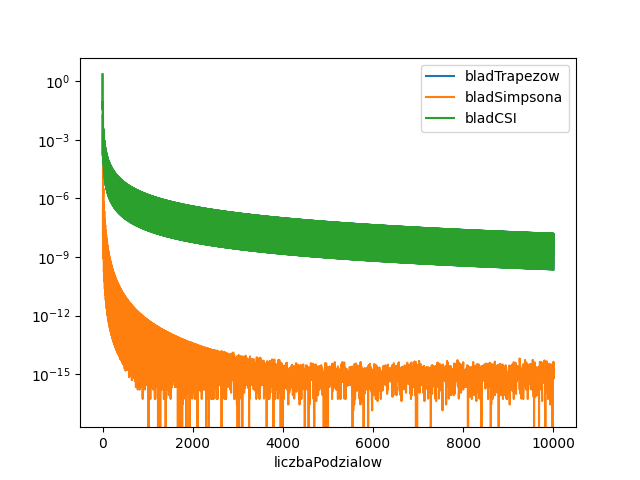
\includegraphics[width=11cm]{alg_num_zad3.png}
    \caption{Zestawienie błędów wszystkich metod wykonanych na podanych funkcjach z różnymi ilościami węzłów.}
    \label{fig:bledy}
\end{figure}

\subsection{Hipoteza 1 - Druga metoda daje dokładniejsze wyniki niż pierwsza }

Ta hipoteza jest potwierdzona przez wykres \ref{fig:bledy}, gdzie niebieska linia, reprezentująca błędy metody trapezów, przesłonięta przez zieloną linię, ma większe wartości, niż linia pomarańczowa, reprezentująca metodę Simpsona.

\subsection{Hipoteza 2 - Trzecia metoda daje dokładniejsze wyniki niż druga }

Odrzucono tą hipotezę, gdyż zielona linia na wykresie \ref{fig:bledy}, reprezentująca błędy metody CSI, w pełni pokrywa się z błędami metody trapezów, jednocześnie mając większe błędy niż metoda Simpsona. Przyglądając się poszczególnym wartościom błędów widać niewielkie różnice między błędami metody CSI a trapezów, niemniej jest to niepokojące i taki stan rzeczy najprawdopodobniej wynika z błędnej implementacji. Błędy przy wyliczaniu macierzy prawdopodobnie nie powodują nieprawidłowych wyników, ponieważ są one wystarczająco małe, by nie brać ich pod uwagę i nie powinny kaskadowo wywoływać tak dużych błędów przy całkowaniu metodą CSI. Wyklucza się taką możliwość, gdyż w ten sposób wywołane błędy w całkowaniu nie pokrywałyby się w takim stopniu z błędami metody trapezów.

\subsection{Hipoteza 3 - Błędy maleją wraz ze wzrostem liczby węzłów}

Wartości wszystkich funkcji na wykresie \ref{fig:bledy} maleją wraz ze wzrostem liczby węzłów, w związku z czym hipoteza jest udowodniona.

\section{Podsumowanie}

Dwie z powyższych hipotez zostały potwierdzone, jednak implementacja metody CSI najprawdopodobniej zawiera błędy, sądząc po wynikach odbiegających od oczekiwań. Metoda Simpsona cechuje się dość małymi błędami, co można uznać za sukces.

\end{document}
